\section{Experiments}
\label{sec:experiments}

\subsection{Experimental Setup}

\paragraph{Datasets and metrics.}
FashionIQ contains three categories, dress, shirt, and toptee, and evaluates retrieval from a reference garment and two natural-language modifications~\cite{wufashioniq}. Following the directly comparable validation protocol, we exclude the source image and report the category mean of \Rten and \Rfifty. FashionGen is evaluated through the FashionMV validation protocol~\cite{yuan2026fashionmv}, with 9,031 composed queries and 5,292 gallery products. We report \Rone, \Rfive, and \Rten. CIRR contains natural images from diverse domains and evaluates a reference image paired with one relative caption~\cite{liucirr}. We report global \Rone, \Rfive, \Rten, and \Rfifty; subset recall at ranks 1, 2, and 3; and $\mathrm{Avg}=(\Rfive+\text{subset }\Rone)/2$.

\paragraph{Endpoints.}
For FashionIQ, our primary pair combines the author-released MCoT-MVS endpoint~\cite{ge2026mcot} with reproduced DQU-CIR endpoints~\cite{wen2024dqu}. We evaluate DQU Base and a GradCache effective-batch-128 checkpoint. Every local method uses the same gallery convention and stable source exclusion. For FashionGen, we use two independently trained 0.8B ProCIR-compatible A1 endpoints based on the public FashionMV code~\cite{yuan2026fashionmv}. CIRR pairs the released MCoT endpoint with a DQU endpoint trained from the authors' recipe. The diagonal ensemble and \method always encode the same two queries and two gallery representations.

\paragraph{Implementation.}
Embeddings are $\ell_2$ normalized before scoring. The FashionIQ cross mean is fully parameter free. The FashionGen router uses 17 actions, hidden width 128, three epochs, and regression cost $\lambda=2$. Training and threshold selection use only the internal split; the reported validation ranking is produced by the frozen router. On CIRR, the target-refinement head reranks the top 50 global candidates and the subset members. It uses eight segment tokens per image, hidden width 512, and eight training epochs; the best frozen checkpoint is followed by the fixed $\alpha=0.25$ score in Eq.~\ref{eq:weakpath}. All recall values are percentages. Gallery encoding is offline, and experiments run on one RTX 4090.

\subsection{Main Results}

\begin{table}[t]
\centering
\caption{\textbf{FashionGen results under the FashionMV validation protocol.} Public baselines are reported by FashionMV~\cite{yuan2026fashionmv}. The diagonal ensemble is compute matched to our method. Best local results are bold.}
\label{tab:fashiongen}
\scriptsize
\setlength{\tabcolsep}{1.8pt}
\begin{tabular}{llccc}
\toprule
Method & Venue/src. & \Rone & \Rfive & \Rten \\
\midrule
CLIP4CIR & CVPR'22 & -- & 17.10 & 25.00 \\
SPRC & FMV'26 & -- & 42.70 & 53.00 \\
Qwen3-VL-2B & FMV'26 & -- & 63.00 & 74.10 \\
Qwen3-VL-8B & FMV'26 & -- & 74.70 & 83.50 \\
Doubao-E-V & FMV'26 & -- & 67.20 & 77.10 \\
ProCIR & arXiv'26 & -- & 75.00 & 85.30 \\
\midrule
A1 reproduced base & Local & 42.73 & 79.26 & 87.75 \\
Diagonal ensemble & Local & 42.85 & 79.74 & 88.24 \\
Cross mean (ours) & Local & \best{44.10} & 79.74 & 88.16 \\
\method joint routing (ours) & Local & 44.09 & \best{80.36} & \best{88.28} \\
\bottomrule
\end{tabular}
\end{table}

Table~\ref{tab:fashiongen} shows that the reproduced A1 endpoint exceeds the published ProCIR result by 4.26 \Rfive and 2.45 \Rten. Running a second endpoint and averaging only the diagonal gives modest gains. The cross mean raises \Rone from 42.73 to 44.10, exceeding the diagonal ensemble by 1.25 points. Joint routing retains almost all of this early-rank gain and reaches 80.36 \Rfive and 88.28 \Rten. Relative to the base, the improvement is 1.36, 1.10, and 0.53 points. Paired bootstrap confidence intervals for these gains are $[0.96,1.68]$, $[0.84,1.34]$, and $[0.30,0.74]$, respectively.

\begin{table}[t]
\centering
\caption{\textbf{FashionIQ validation results.} Paper values use their published protocol. Local results are recomputed in one source-excluded pipeline. Diagonal is compute matched.}
\label{tab:fashioniq}
\small
\setlength{\tabcolsep}{3.2pt}
\begin{tabular}{llcc}
\toprule
Method & Venue & \Rten & \Rfifty \\
\midrule
TIRG~\cite{vo2019tirg} & CVPR'19 & 17.40 & 37.39 \\
CLIP4CIR~\cite{baldrati2022clip4cir} & CVPR'22 & 38.40 & 61.74 \\
CCIN~\cite{tian2025ccin} & CVPR'25 & 54.41 & 74.76 \\
DQU-CIR~\cite{wen2024dqu} & SIGIR'24 & 62.00 & 81.58 \\
MCoT-MVS~\cite{ge2026mcot} & WWW'26 & 63.24 & 82.01 \\
\midrule
MCoT-MVS, same pipeline & Local & 63.56 & 82.33 \\
Diagonal ensemble & Local & 64.52 & 82.75 \\
Cross mean, Base $\times$ MCoT (ours) & Local & \best{64.61} & 82.57 \\
Cross mean, GC $\times$ MCoT (ours) & Local & 64.58 & \best{82.82} \\
\bottomrule
\end{tabular}
\end{table}

FashionIQ provides a heterogeneous test: DQU performs raw-data fusion, whereas MCoT uses multimodal reasoning and hierarchical visual selection. Table~\ref{tab:fashioniq} shows that this difference is useful after training. DQU Base with MCoT obtains the highest \Rten at 64.61. Replacing DQU Base with the GradCache endpoint gives the highest \Rfifty at 82.82. The latter improves the same-pipeline MCoT endpoint by 1.02 \Rten and 0.48 \Rfifty. It also exceeds the compute-matched diagonal ensemble at both cutoffs. Under the include-source convention of the released MCoT evaluator, the corresponding gain is 1.21 \Rten and 0.55 \Rfifty, confirming that the improvement is not tied to source handling.

\begin{table*}[t]
\centering
\caption{\textbf{CIRR validation results in one aligned pipeline.} Subset denotes the six-image candidate group. The best result in each column is bold.}
\label{tab:cirr}
\small
\setlength{\tabcolsep}{4.1pt}
\begin{tabular}{lcccccccc}
\toprule
Method & \Rone & \Rfive & \Rten & \Rfifty & Subset R@1 & Subset R@2 & Subset R@3 & Avg \\
\midrule
MCoT, same pipeline & 54.94 & 85.27 & 91.89 & \best{98.49} & 78.02 & 91.94 & 96.68 & 81.64 \\
\method, $\alpha=0.25$ & 55.23 & 85.36 & 92.32 & 98.40 & \best{79.02} & 92.08 & \best{96.99} & 82.19 \\
\method + target refinement & \best{55.78} & \best{85.77} & \best{92.42} & 98.40 & 79.00 & \best{92.15} & \best{96.99} & \best{82.38} \\
\bottomrule
\end{tabular}
\end{table*}

\paragraph{Open-domain transfer.}
Table~\ref{tab:cirr} extends CrossPath beyond fashion retrieval. Conservative fusion raises CIRR Avg from 81.64 to 82.19, with gains in global recall through rank 10 and all subset metrics. Query-conditioned target refinement reaches 55.78 \Rone, 85.77 \Rfive, and 82.38 Avg. The combined model improves the frozen MCoT endpoint by 0.84 \Rone, 0.50 \Rfive, and 0.74 Avg. Weak fusion obtains the highest subset \Rone, while target refinement improves the global top ranks and subset ranks 2 and 3. These complementary changes support the staged design in Sec.~\ref{sec:conservative}.

\subsection{Component Analysis}

\begin{figure}[t]
    \centering
    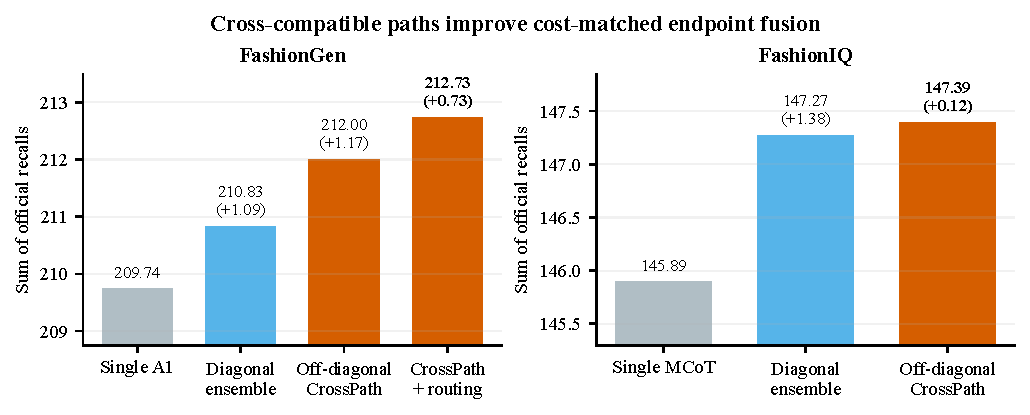
\includegraphics[width=\columnwidth]{figures/fig_positive_module_ablation.pdf}
    \caption{\textbf{Cumulative component ablation.} FashionGen uses $\Rone+\Rfive+\Rten$; FashionIQ uses $\Rten+\Rfifty$. Every added component yields a positive gain.}
    \label{fig:ablation}
\end{figure}

Figure~\ref{fig:ablation} starts from the strongest single endpoint and adds one component at a time. On FashionGen, the diagonal ensemble contributes 1.09 SumR, off-diagonal compatibility adds 1.17, and routing adds another 0.73. The final SumR improves from 209.74 to 212.73. On FashionIQ, the diagonal ensemble contributes 1.38 and replacing diagonal-only fusion with cross paths adds 0.12, reaching 147.39. The smaller final step is consistent with an already strong heterogeneous ensemble, but it is obtained without fusion training.

\begin{figure}[t]
    \centering
    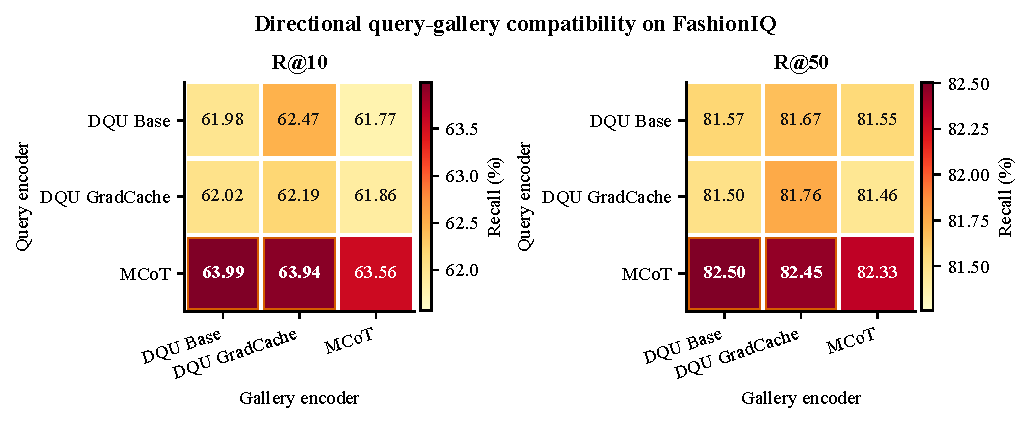
\includegraphics[width=\columnwidth]{figures/fig_fashioniq_compatibility_matrix.pdf}
    \caption{\textbf{Directional FashionIQ compatibility.} Each cell pairs the row query encoder with the column gallery encoder and reports \Rten/\Rfifty. Off-diagonal strength is concentrated in MCoT queries paired with DQU galleries.}
    \label{fig:matrix}
\end{figure}

\paragraph{Directionality.}
Figure~\ref{fig:matrix} expands the analysis to three endpoints. MCoT queries paired with DQU Base and DQU GradCache galleries reach 63.99/82.50 and 63.94/82.45. Both improve over the MCoT diagonal at 63.56/82.33. The reverse DQU-query to MCoT-gallery directions are weaker, ranging from 61.77 to 61.86 \Rten. Cross compatibility is therefore structured and directional, not an automatic consequence of pairing arbitrary endpoint outputs.

\begin{table}[t]
\centering
\caption{\textbf{Coordinate-scrambling control.} A shared signed permutation preserves all within-endpoint dot products and diagonal rankings, while breaking cross-endpoint coordinates.}
\label{tab:scramble}
\small
\setlength{\tabcolsep}{4.3pt}
\begin{tabular}{lccc}
\toprule
Dataset and path & \Rone & \Rten & \Rfifty \\
\midrule
FashionIQ cross & -- & 64.58 & 82.82 \\
FashionIQ scrambled & -- & 0.85 & 3.08 \\
\midrule
FashionGen cross & 44.10 & 88.16 & -- \\
FashionGen scrambled & 0.14 & 0.95 & -- \\
\bottomrule
\end{tabular}
\end{table}

\paragraph{Compatibility intervention.}
Table~\ref{tab:scramble} reports the signed-permutation test from Sec.~\ref{sec:method}. The maximum change in any preserved endpoint score is $7.75\times10^{-7}$ on FashionGen and $3.58\times10^{-7}$ on FashionIQ. Thus each endpoint and the diagonal ensemble retain their rankings up to floating-point precision. Cross-path performance nevertheless collapses from 64.58/82.82 to 0.85/3.08 on FashionIQ and from 44.10/79.74/88.16 to 0.14/0.59/0.95 on FashionGen. The useful signal is carried by aligned cross-endpoint coordinates.

\paragraph{Rescue and regression.}
At the principal cutoffs, cross paths rescue more base failures than they harm base successes. FashionGen has 294 rescues versus 170 regressions at rank 1, 169 versus 126 at rank 5, and 125 versus 88 at rank 10. FashionIQ has 218 versus 170 at rank 1, 199 versus 138 at rank 10, and 121 versus 92 at rank 50. This balance explains why a simple mean is effective and why cutoff-aware routing provides an additional gain on FashionGen.

\subsection{Efficiency}

\begin{table}[t]
\centering
\caption{\textbf{Additional CrossPath cost.} Gallery storage is for two FP32 embedding sets. Query time excludes offline gallery encoding and gallery dot products.}
\label{tab:efficiency}
\small
\setlength{\tabcolsep}{3.0pt}
\begin{tabular}{lccc}
\toprule
Setting & Params & Gallery & Time/query \\
\midrule
FashionIQ cross mean & 0 & 22.45 MiB & 55.44 ms \\
FashionGen joint & 0.526M & 41.34 MiB & 4.48 ms$^{\dagger}$ \\
\bottomrule
\end{tabular}
\vspace{2pt}
\raggedright\scriptsize $^{\dagger}$Post-embedding router and policy time on an RTX 4090.
\end{table}

The FashionIQ cross mean adds no trainable fusion parameter. Its 55.44 ms query time is the sum of MCoT and DQU query encoding; gallery representations are computed once. The FashionGen router adds 0.526M parameters and 4.48 ms per query after embedding. It examines only 0.37, 2.02, and 3.85 boundary candidates per query on average at ranks 1, 5, and 10. The method returns a single ranking and does not require repeated retrieval passes.

\subsection{Qualitative Results}

\begin{figure*}[t]
    \centering
    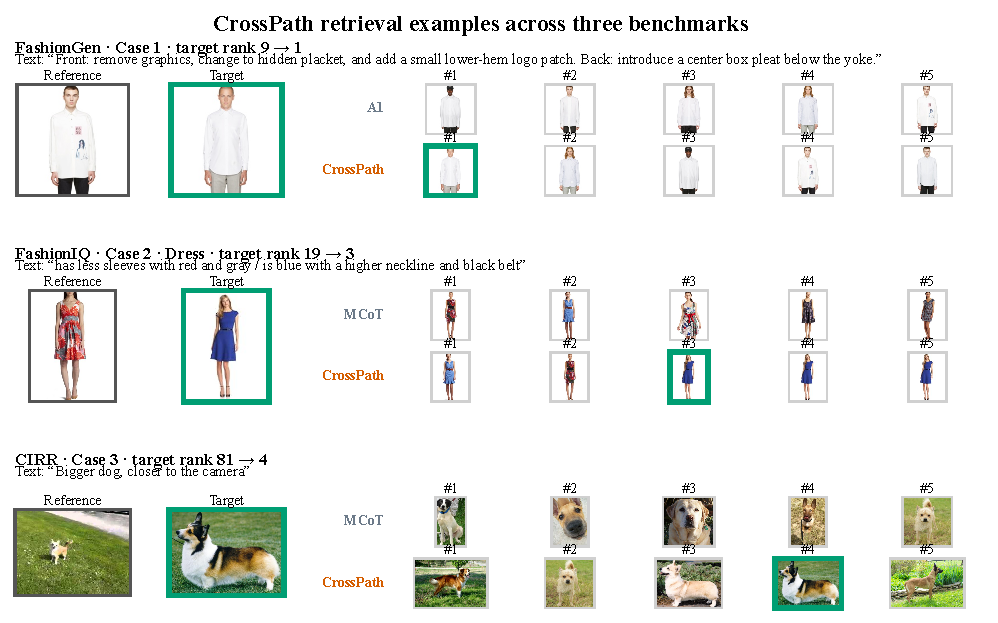
\includegraphics[width=\textwidth]{figures/fig_crosspath_retrieval_cases.pdf}
    \caption{\textbf{Retrieval examples across FashionGen, FashionIQ, and CIRR.} Each query shows the reference, modification, target, and top-five results from the base endpoint and \method. Green borders mark the target.}
    \label{fig:qualitative}
\end{figure*}

Figure~\ref{fig:qualitative} illustrates the quantitative trend on all three benchmarks. The base endpoint often retrieves visually plausible images that retain dominant reference content but miss the requested edit. Cross paths promote targets that better satisfy both the retained appearance and the modification. Cases are selected deterministically by the largest base-miss to CrossPath-hit rank improvement, with no manual visual screening. The figure pipeline reads the original benchmark files; no image is generated or upsampled.
